% NGISE 2026 proceedings version (Springer LNCS template, limit 12 pages).
% Full version with all proofs: arXiv:2608.05316.
% Build: make  (pdflatex + bibtex via latexmk)
\documentclass[runningheads]{llncs}

\usepackage[T1]{fontenc}
\usepackage{amsmath}
\usepackage{newtxtext}
\usepackage[varvw]{newtxmath}
\usepackage{graphicx}
\usepackage{booktabs}
\usepackage{array}
\usepackage{tikz}
\usetikzlibrary{arrows.meta,positioning,calc}
\usepackage{color}
\usepackage[hidelinks]{hyperref}
\renewcommand\UrlFont{\color{blue}\rmfamily}
\urlstyle{rm}

% ---------------------------------------------------------------- notation
\newcommand{\LeafHash}{\mathsf{LeafHash}}
\newcommand{\NodeHash}{\mathsf{NodeHash}}
\newcommand{\PreHash}{\mathsf{HashPreState}}
\newcommand{\dig}{\mathsf{dig}}
\newcommand{\Tree}{\mathsf{Tree}}
\newcommand{\Leaf}{\mathsf{Leaf}}
\newcommand{\Node}{\mathsf{Node}}
\newcommand{\Empty}{\mathsf{Empty}}
\newcommand{\reg}{\mathsf{reg}}
\newcommand{\dep}{\mathsf{dep}}
\newcommand{\map}{\mathsf{map}}
\newcommand{\ins}{\mathsf{ins}}
\newcommand{\nxt}{\mathsf{next}}
\newcommand{\lcp}{\mathsf{lcp}}
\newcommand{\eval}{\mathsf{eval}}
\newcommand{\Hole}{\mathsf{Hole}}
\newcommand{\OLeaf}{\mathsf{OLeaf}}
\newcommand{\ONode}{\mathsf{ONode}}
\newcommand{\Certify}{\mathsf{Certify}}
\newcommand{\dom}{\mathrm{dom}}
\newcommand{\cat}{\mathbin{\|}}
\newcommand{\K}{\mathcal{K}}
\newcommand{\V}{\mathcal{V}}
\newcommand{\bits}[1]{\texttt{#1}}

% ---------------------------------------------------------------- figures
\definecolor{preserved}{HTML}{E2E4E7}
\definecolor{opened}{HTML}{FFFFFF}
\definecolor{fresh}{HTML}{FBC9A6}
\definecolor{recomp}{HTML}{FDEBDD}
\definecolor{attack}{HTML}{F6C4C5}
\definecolor{attackline}{HTML}{C0282D}
\definecolor{accent}{HTML}{F25F05}
\definecolor{lineGrey}{HTML}{585A5E}

\tikzset{
  box/.style={draw=lineGrey, rounded corners=2pt, align=center, inner sep=2.5pt, font=\footnotesize},
  jn/.style={box, minimum width=1.6cm, minimum height=0.55cm},
  lf/.style={box, minimum width=1.35cm, minimum height=0.55cm},
  arr/.style={-{Latex[length=1.8mm]}, semithick, lineGrey},
  lbl/.style={font=\scriptsize, inner sep=1.5pt},
  bitlbl/.style={font=\scriptsize, inner sep=1pt},
  ord/.style={font=\scriptsize\bfseries, text=accent, inner sep=1pt},
}
\newcommand{\swatch}[1]{\tikz[baseline=-0.6ex]\node[box, fill=#1, minimum width=2.5mm, minimum height=2.5mm, inner sep=0]{};}

% ---------------------------------------------------------------- title
\begin{document}

\title{The Trust-Free Aggregation Layer\\ of the Unicity Infrastructure}
\titlerunning{The Trust-Free Aggregation Layer of the Unicity Infrastructure}

\author{Risto Laanoja\inst{1} \and Mike Gault\inst{1} \and Dirk Draheim\inst{2} \and Ahto Buldas\inst{2}}
\authorrunning{R. Laanoja et al.}
% TODO: e-mail addresses, postal addresses, ORCID iDs
\institute{Unicity Labs \and Tallinn University of Technology, Tallinn, Estonia}

\maketitle
\setcounter{footnote}{0}

\begin{abstract}
The Unicity Network executes and validates token transactions off-chain, between the parties involved, and keeps one globally shared object: a record of consumed token states. Offline checks, including computational integrity proofs, cannot establish that a state has not been consumed before, because a state and its proof can be copied. This record is therefore the minimal online component of a trustless peer-to-peer transaction system. We present it as an add-only authenticated dictionary that is operated by an untrusted aggregator and certified, round by round, by a consensus layer that checks a consistency proof. The dictionary is a radix sparse Merkle tree whose junction hashes commit to their absolute depth and key prefix. Inclusion and non-inclusion share one certificate format with one sibling digest per junction on the key path. We prove that a non-inclusion certificate determines the root after the key is inserted, so that a run of single insertions is append-only consistent under collision resistance of the hash function alone. For batches we give a five-opcode transcript language whose verifier checks key placement locally, show why this check is necessary, and state the soundness theorem for certified histories, whose full proof is in the extended version.
------ver 2-----
The Unicity Network executes and validates token transactions off-chain, directly between the parties involved, without the transaction validator network and shared ledger overhead. The only global coordination is a record of consumed token states: information theoretically, one can not establish if a data object is copied or not without shared coordination. We present such coordinator as an authenticated dictionary that can be operated by an untrusted entity. The authenticator is certified, round by round, by a consensus layer that checks the validity of its state transitions. We prove that a non-inclusion certificate determines the root after the key is inserted, so that a run of single insertions is append-only consistent under collision resistance of the hash function alone. To prove it for batches, we give a five-opcode transcript language whose verifier checks key placement locally, show why this check is necessary, and state the soundness theorem for certified histories, whose full proof is in the extended version.

\keywords{Authenticated data structures \and Sparse Merkle trees \and Double-spending \and Blockchain}
\end{abstract}

% =====================================================================
\section{Introduction}
% =====================================================================

A legacy blockchain orders and executes all transactions in one replicated state machine. The Unicity Network~\cite{wp} takes the opposite approach. Tokens are self-contained data objects kept by their owners, and a transaction is executed and validated off-chain by the counterparties~\cite{exemodel}. A recipient checks the token history offline: signatures, spending predicates, and optionally a computational integrity proof of a longer computation.

Offline checks cannot establish that a state has not been consumed before. Cryptography alone, like a succinct proof $\pi$ can attest that a state $s$ results from a valid computation, but not that the pair $(s,\pi)$ is the unique copy. Data can be copied, and all instances can be continued by transitions $s \to s'$ and $s \to s''$ with valid proofs (Fig.~\ref{fig:model}a). This is a double-spend, or a fork of the token. Excluding it requires a certificate that $s$ was consumed at most once, which is a statement about global view. A trustless peer-to-peer system therefore needs something like an online, shared record of consumed states, with cryptographic inclusion and non-inclusion proofs against a unique certified root.\footnote{Other options are trusted hardware (secure elements, TEEs), interacting recipient set, global ordering, etc.} Unicity keeps only this record online and leaves ordering, execution, and data storage to the transacting parties. We call the record the \emph{minimal online component}.

In Unicity the record is maintained by the Aggregation Layer. A key $k = H(\text{state})$ identifies a consumed token state, and its value $v = H(\text{transaction})$ identifies the transaction that consumed it. A transaction is accepted only together with its \emph{proof of unicity}, an inclusion proof of $k \mapsto v$ against a root certified by the Consensus Layer. The aggregator is not trusted. In every round it submits the previous root, the new root, and a consistency proof; and the Consensus Layer certifies the new root only if the proof verifies (Fig.~\ref{fig:model}b). This paper is about the data structure and the proofs that make this arrangement trustless. Our contributions are:
\begin{itemize}
  \item a formulation of the record as an add-only authenticated dictionary with inclusion, non-inclusion, and consistency proofs, and of its security as a reduction to collision resistance (Sect.~\ref{sec:model});
  \item the region-committing radix sparse Merkle tree (RSMT), in which every finite map has exactly one valid tree and inclusion and non-inclusion share one certificate with one sibling digest per junction on the key path (Sect.~\ref{sec:rsmt});
  \item a proof that a non-inclusion certificate determines the root after insertion and transforms into the inclusion certificate of the new binding, so that certified runs of single insertions are append-only consistent (Sect.~\ref{sec:single});
  \item an opcode-based transcript language for proving batch insertion consitency with a one-pass verifier that checks key placement locally, and the soundness and completeness theorems for batch rounds (Sect.~\ref{sec:batch}).
\end{itemize}
The extended version of this paper~\cite{fullversion} contains all proofs, the algorithms, the arithmetization of the batch verifier as a STARK, and the recursive aggregation of the full certified history into one proof.

\begin{figure}[t]
\centering
\begin{minipage}[b]{0.47\textwidth}\centering
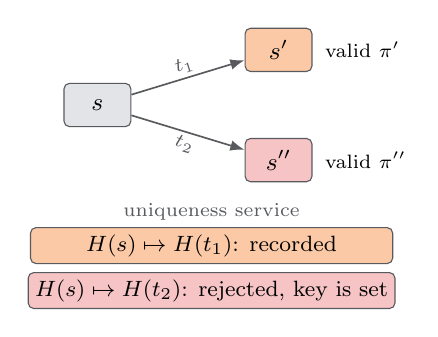
\begin{tikzpicture}[st/.style={box, minimum width=0.85cm, minimum height=0.55cm, font=\small}]
  \node[st, fill=preserved] (s) at (0,0) {$s$};
  \node[st, fill=fresh] (s1) at (2.3,0.7) {$s'$};
  \node[st, fill=attack] (s2) at (2.3,-0.7) {$s''$};
  \draw[arr] (s) -- node[lbl, above, sloped] {$t_1$} (s1);
  \draw[arr] (s) -- node[lbl, below, sloped] {$t_2$} (s2);
  \node[lbl, right=1mm of s1] {valid $\pi'$};
  \node[lbl, right=1mm of s2] {valid $\pi''$};
  \node[box, fill=fresh, anchor=north, minimum width=4.6cm] (r1) at (1.45,-1.55) {$H(s) \mapsto H(t_1)$: recorded};
  \node[box, fill=attack, below=1mm of r1, minimum width=4.6cm] (r2) {$H(s) \mapsto H(t_2)$: rejected, key is set};
  \node[lbl, above=0.3mm of r1, text=lineGrey] {uniqueness service};
\end{tikzpicture}\\[1mm]
{\footnotesize (a)}
\end{minipage}\hfill
\begin{minipage}[b]{0.5\textwidth}\centering
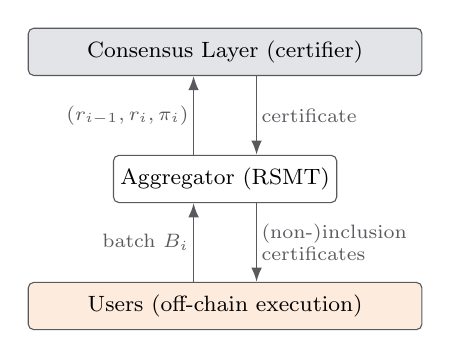
\begin{tikzpicture}
  \node[box, fill=preserved, minimum width=5.0cm, minimum height=0.6cm] (cl) {Consensus Layer (certifier)};
  \node[box, fill=white, minimum width=2.8cm, minimum height=0.6cm, below=1.0cm of cl] (ag) {Aggregator (RSMT)};
  \node[box, fill=recomp, minimum width=5.0cm, minimum height=0.6cm, below=1.0cm of ag] (us) {Users (off-chain execution)};
  \draw[arr] ([xshift=-4mm]ag.north) -- node[lbl, left] {$(r_{i-1}, r_i, \pi_i)$} ([xshift=-4mm]ag.north |- cl.south);
  \draw[arr] ([xshift=4mm]ag.north |- cl.south) -- node[lbl, right] {certificate} ([xshift=4mm]ag.north);
  \draw[arr] ([xshift=-4mm]us.north -| ag.south) -- node[lbl, left] {batch $B_i$} ([xshift=-4mm]ag.south);
  \draw[arr] ([xshift=4mm]ag.south) -- node[lbl, right, align=left] {(non-)inclusion\\certificates} ([xshift=4mm]us.north -| ag.south);
\end{tikzpicture}\\[1mm]
{\footnotesize (b)}
\end{minipage}
\Description{Left: a state s has two transitions, t1 to s' and t2 to s'', each with a valid proof. A uniqueness service records H(s) mapped to H(t1) and rejects H(s) mapped to H(t2) because the key is set. Right: users send a batch to the aggregator and receive inclusion and non-inclusion certificates; the aggregator sends the previous root, the new root, and a consistency proof to the Consensus Layer and receives a certificate.}
\caption{(a) A state and its proof can be copied, and both copies can be continued validly. The uniqueness service records one consumption of $s$ and rejects the other. (b) System model. The aggregator is untrusted; the Consensus Layer certifies $r_i$ only if $\pi_i$ verifies against $(r_{i-1}, r_i)$.}
\label{fig:model}
\end{figure}

% =====================================================================
\section{System Model and Security Goal}\label{sec:model}
% =====================================================================

Let $\K = \{0,1\}^{\kappa}$, $\kappa = 256$, be the key space and $\V$ the value space. After round $i$ the aggregator holds a finite partial map $M_i\colon \K \to \V \cup \{\bot\}$, with $M_0 = \emptyset$, committed by a digest $r_i$. The dictionary is \emph{add-only}: $M_{i-1} \subseteq M_i$, so a key is set at most once and is never changed or removed. Insertion order is not retained, and the digest commits to the map. Three kinds of proof are used (Table~\ref{tab:proofs}).

\begin{table}[t]
\centering
\caption{Proofs provided by the dictionary.}\label{tab:proofs}
\setlength{\tabcolsep}{5pt}
\begin{tabular}{@{}llll@{}}
\toprule
Proof & Statement & Verified against & Verified by \\
\midrule
inclusion & $M_i(k) = v$ & $r_i$ & recipients \\
non-inclusion & $M_i(k) = \bot$ & $r_i$ & recipients \\
consistency & $M_{i-1} \subseteq M_i$ & $(r_{i-1}, r_i)$ & Consensus Layer \\
\bottomrule
\end{tabular}
\end{table}

Requests are processed in batches. At the end of round $i$ the aggregator sends $(r_{i-1}, r_i, \pi_i)$ to the Consensus Layer, which we model as an oracle $\Certify$. It keeps the last certified root $r_{\mathrm{last}}$, initially the digest of the empty map. $\Certify(r_{i-1}, r_i, \pi_i)$ returns $\bot$ unless $r_{i-1} = r_{\mathrm{last}}$ and $\pi_i$ verifies against $(r_{i-1}, r_i)$; otherwise it sets $r_{\mathrm{last}} \gets r_i$ and returns a signed certificate $(i, r_i, r_{i-1}; \sigma)$. Each certified root is extended at most once, so the certified roots form a chain and the dictionary cannot fork. The certifier stores the latest roots only, not a log. In Unicity it is the BFT Core, a validator committee elected by delegated proof of stake~\cite{wp}.

\begin{definition}[Security]\label{def:security}
Let $\mathsf{Dig}(M)$ denote the digest of a map $M$ (Sect.~\ref{sec:rsmt}).
\begin{enumerate}
  \item From any consistency proof that verifies against $(r_{i-1}, r_i)$, partial maps $M_{i-1} \subseteq M_i$ with $\mathsf{Dig}(M_{i-1}) = r_{i-1}$ and $\mathsf{Dig}(M_i) = r_i$ are efficiently computable, or a collision of $H$ is.
  \item From two proofs for $M(k) = v$ and $M(k) = v'$ with $v \neq v'$ that verify against the same digest, a collision of $H$ is efficiently computable.
\end{enumerate}
\end{definition}

Under Definition~\ref{def:security} the adversarial aggregator can affect only liveness. It can delay or censor requests, which replicated aggregators and resubmission mitigate, and the omission of an accepted request is detected when the recipient asks for an inclusion certificate against the certified root. It cannot change or remove a recorded binding. The certifier's quorum is trusted for liveness and for the uniqueness of the latest root. A quorum that signs two continuations of one root leaves attributable evidence; no proof system can exclude it. The extended version~\cite{fullversion} removes the quorum from the correctness argument for the recorded history by aggregating all consistency proofs into one recursive STARK.

% =====================================================================
\section{The Radix Sparse Merkle Tree}\label{sec:rsmt}
% =====================================================================

A sparse Merkle tree~\cite{merkle1987,dahlberg2016smt} assigns every key a leaf of a binary tree of depth $\kappa$; all empty subtrees are implicit. Its radix variant, a binary Patricia trie~\cite{morrison1968}, contains only leaves and junctions (bifurcations). For $n$ uniformly distributed keys the expected root-to-leaf path length is $\log_2 n + O(1)$, while no binary tree with $n$ leaves has a mean leaf depth below $\log_2 n$. A certificate with one sibling digest per junction on the path is therefore within an additive constant of the optimum.

\paragraph{Notation.} For bit strings, $p \preceq q$ states that $p$ is a prefix of $q$, $q[j]$ is bit $j$ (counted from $0$), $q[0..d)$ is the prefix of length $d$, $\lcp(x,y)$ is the longest common prefix, and $\varepsilon$ is the empty string. $H\colon \{0,1\}^* \to \{0,1\}^{\lambda}$ is the hash function, $\langle\cdot\rangle$ are fixed-length one-to-one encodings, and $\varnothing$ is a constant outside $\{0,1\}^{\lambda}$ that marks an empty tree. All statements below are reductions: each concludes the stated property, or that a collision of $H$ is computable in time linear in the size of the objects involved.

A leaf hashes the full key with the value, and a junction hashes its children $x, y$ with its depth $d$ and its \emph{region} $p \in \{0,1\}^{d}$, the prefix shared by all keys below it:
\begin{align*}
  \LeafHash(k,v) &= H(\texttt{0x00} \cat k \cat v),\\
  \NodeHash(d,p,x,y) &= H(\texttt{0x01} \cat \langle d\rangle \cat \langle p\rangle \cat x \cat y).
\end{align*}
Depth and region are absolute properties of a node. Inserting a key splits an edge above a node while not changing their properties, thus an insertion does not change the hashes of existing nodes.

\begin{definition}[Valid trees]\label{def:tree}
Trees are $\Empty$, $\Leaf(k,v)$, and $\Node(d,p,T_l,T_r)$ with $k \in \K$, $v \in \V$, $0 \le d < \kappa$, $p \in \{0,1\}^{d}$. The digest is $\dig(\Empty) = \varnothing$, $\dig(\Leaf(k,v)) = \LeafHash(k,v)$, and $\dig(\Node(d,p,l,r)) = \NodeHash(d,p,\dig(l),\dig(r))$. A leaf has region $k$ and depth $\kappa$; a junction has region $p$ and depth $d$. A tree is \emph{valid} if every junction $\Node(d,p,l,r)$ in it has nonempty children with $\dep(l), \dep(r) > d$, $p \cat \bits{0} \preceq \reg(l)$, and $p \cat \bits{1} \preceq \reg(r)$.
\end{definition}

The validity conditions are local, one per edge. Global consequences are the following.

\begin{lemma}[Shape]\label{lem:shape}
In a valid tree $T$: (i) every leaf key extends the region of each ancestor, and distinct leaves carry distinct keys, so $T$ represents the map $\map(T) = \{k \mapsto v \mid \Leaf(k,v) \in T\}$; (ii) the region of every junction is the longest common prefix of the keys below it; (iii) the left-to-right order of leaves is the increasing order of keys.
\end{lemma}
\begin{proof}
(i) follows by induction from $p \cat \beta \preceq \reg(\text{child})$ on every edge; two leaves with equal key would lie on opposite sides of their lowest common ancestor. (ii) Both children are nonempty and their keys differ at bit $d$. (iii) At each junction, keys on the left have bit $0$ and keys on the right bit $1$ at position $d$.\qed
\end{proof}

\begin{proposition}[Unique representation]\label{prop:unique}
Every finite partial map $M$ has exactly one valid tree, written $\Tree(M)$. We set $\mathsf{Dig}(M) = \dig(\Tree(M))$.
\end{proposition}
\begin{proof}
Write $M_q = \{k \mapsto v \in M \mid q \preceq k\}$. Induction on $|\dom(M)|$: the empty map gives $\Empty$ and a singleton gives its leaf. Otherwise let $p$ be the longest common prefix of $\dom(M)$. The maps $M_{p\cat 0}$ and $M_{p\cat 1}$ are nonempty, have unique valid trees by induction, and $\Node(|p|, p, \Tree(M_{p\cat 0}), \Tree(M_{p\cat 1}))$ is valid. Conversely, Lemma~\ref{lem:shape}(ii) forces the root region of any valid tree for $M$ to be $p$, validity forces its children to represent $M_{p\cat 0}$ and $M_{p\cat 1}$, and induction forces the children.\qed
\end{proof}

All arguments below rest on one lemma about partially opened commitments.

\begin{definition}[Opening trees]\label{def:opening}
Opening trees are $\Hole(c)$, $\OLeaf(k,v)$, and $\ONode(d,p,F_l,F_r)$ with $c \in \{0,1\}^{\lambda}$ and the other operands as in Definition~\ref{def:tree}. Evaluation mirrors $\dig$, with $\eval(\Hole(c)) = c$.
\end{definition}

\begin{lemma}[Matching]\label{lem:match}
Let $T \neq \Empty$ and let $F$ be an opening tree with $\eval(F) = \dig(T)$. Then every $\ONode(d,p,\cdot,\cdot)$ and $\OLeaf(k,v)$ of $F$ coincides with a node $\Node(d,p,\cdot,\cdot)$ or $\Leaf(k,v)$ of $T$ at the same position, every $\Hole(c)$ is at the position of a subtree of $T$ with digest $c$, and replacing each hole by that subtree turns $F$ into $T$.
\end{lemma}
\begin{proof}
Induction on $F$ with the invariant $\eval(F) = \dig(T)$. A hole is assigned the current subtree of $T$. Otherwise the two $H$-preimages are equal, or they form a collision. Equal preimages have the same domain tag and, since the encodings are one-to-one, the same constructor and components, and the induction continues in both children.\qed
\end{proof}

\begin{definition}[Certificates]\label{def:cert}
A certificate is the empty certificate $C_\emptyset$ or a sequence of junction openings followed by a terminal leaf,
\[
  C = \big((d_1,s_1),\ldots,(d_m,s_m);\ (k',v')\big), \qquad \kappa > d_1 > \cdots > d_m \ge 0,\ s_j \in \{0,1\}^{\lambda},
\]
listed from the leaf toward the root. To verify $C$ for a target key $k$ against $r$, set $c_0 = \LeafHash(k',v')$ and, for $j = 1,\ldots,m$, require $k[d_j] = k'[d_j]$ and compute $c_j = \NodeHash(d_j,p_j,c_{j-1},s_j)$ if $k'[d_j] = 0$ and $c_j = \NodeHash(d_j,p_j,s_j,c_{j-1})$ otherwise, where $p_j = k'[0..d_j)$. Accept iff all requirements hold and $c_m = r$. $C_\emptyset$ accepts iff $r = \varnothing$. An accepting $C$ is an \emph{inclusion certificate} for $(k,v)$ if $(k',v') = (k,v)$, and a \emph{non-inclusion certificate} for $k$ if $k' \neq k$; $C_\emptyset$ is a non-inclusion certificate for every key.
\end{definition}

The regions are not stored in certificates as they are computable from the terminal key $k'$. (Specifically $k'$, because below the point where $k$ leaves the recorded key space the regions on the path are not prefixes of $k$). The requirement $k[d_j] = k'[d_j]$ ties the path to $k$: the key-directed descent for $k$, which at $\Node(d,p,l,r)$ enters the child on side $k[d]$, traverses the openings. Wrapping $\OLeaf(k',v')$ once per opening, with $\Hole(s_j)$ on the side away from $k'$, gives an opening tree $F_C$ with $\eval(F_C) = c_m$.

\begin{theorem}[Certificate correctness]\label{thm:cert}
Let $T = \Tree(M)$ and let a certificate $C$ verify for $k$ against $\dig(T)$.
\begin{enumerate}
  \item If $C = C_\emptyset$ then $M = \emptyset$. Otherwise $M(k') = v'$; hence $M(k) = v'$ if $k' = k$, and $k \notin \dom(M)$ if $k' \neq k$.
  \item Conversely, for every $k$ a certificate that verifies for $k$ against $\dig(T)$, with terminal key $k$ iff $k \in \dom(M)$, is constructed by one root-to-leaf descent in $T$.
\end{enumerate}
\end{theorem}
\begin{proof}
(i) $C_\emptyset$ verifies only against $\varnothing$, so $T = \Empty$. Otherwise $\eval(F_C) = \dig(T)$, and Lemma~\ref{lem:match} places $\OLeaf(k',v')$ at a leaf of $T$, so $M(k') = v'$, and places every opening at the junction of $T$ at the same position. The openings are therefore ancestors of $\Leaf(k',v')$. If $k \in \dom(M)$, the descent for $k$ ends at $\Leaf(k, M(k))$, because by Lemma~\ref{lem:shape}(i) and validity the child containing that leaf is the one on side $k[d]$. Since $k[d_j] = k'[d_j]$, the same descent follows the openings and ends at $\Leaf(k',v')$, so $k' = k$. Hence $k' \neq k$ implies $k \notin \dom(M)$. (ii) Record the depth and sibling digest of every junction passed by the descent for $k$, and the leaf at which it ends~\cite{fullversion}.\qed
\end{proof}

% =====================================================================
\section{Single Insertion}\label{sec:single}
% =====================================================================

In the simplest round the aggregator records one binding $(k,v)$ and presents a non-inclusion certificate $C$ for $k$. The verifier checks $C$ against $r_{i-1}$ and computes $r_i$ from $C$ itself. The new root is not supplied by the aggregator. Figure~\ref{fig:insert} shows an example with 4-bit keys.

\begin{figure}[t]
\centering
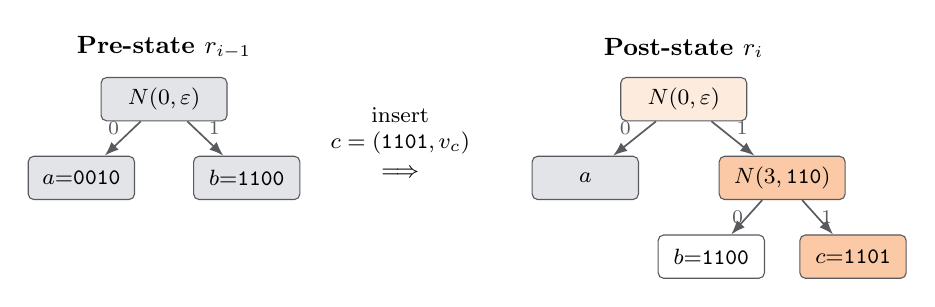
\begin{tikzpicture}[x=1cm,y=1cm]
  \node[font=\small\bfseries] at (0,0.65) {Pre-state $r_{i-1}$};
  \node[jn, fill=preserved] (o) at (0,0) {$N(0,\varepsilon)$};
  \node[lf, fill=preserved] (oa) at (-1.05,-1.0) {$a{=}\bits{0010}$};
  \node[lf, fill=preserved] (ob) at (1.05,-1.0) {$b{=}\bits{1100}$};
  \draw[arr] (o) -- node[bitlbl, above left] {0} (oa);
  \draw[arr] (o) -- node[bitlbl, above right] {1} (ob);
  \node[align=center, font=\footnotesize] at (3.0,-0.55) {insert\\$c = (\bits{1101}, v_c)$\\[1pt]$\Longrightarrow$};
  \node[font=\small\bfseries] at (6.6,0.65) {Post-state $r_i$};
  \node[jn, fill=recomp] (n) at (6.6,0) {$N(0,\varepsilon)$};
  \node[lf, fill=preserved] (na) at (5.35,-1.0) {$a$};
  \node[jn, fill=fresh] (nj) at (7.85,-1.0) {$N(3,\bits{110})$};
  \node[lf, fill=opened] (nb) at (6.95,-2.0) {$b{=}\bits{1100}$};
  \node[lf, fill=fresh] (nc) at (8.75,-2.0) {$c{=}\bits{1101}$};
  \draw[arr] (n) -- node[bitlbl, above left] {0} (na);
  \draw[arr] (n) -- node[bitlbl, above right] {1} (nj);
  \draw[arr] (nj) -- node[bitlbl, left] {0} (nb);
  \draw[arr] (nj) -- node[bitlbl, right] {1} (nc);
\end{tikzpicture}
\Description{Pre-state tree: root junction at depth 0 over leaves a with key 0010 and b with key 1100. Post-state tree after inserting c with key 1101: the root keeps leaf a on its 0-side and has a new junction at depth 3 with region 110 on its 1-side, over leaves b and c.}
\caption{Inserting $c$ with 4-bit keys. A junction $N(d,p)$ shows its depth and region. The descent for $k_c = \bits{1101}$ in the pre-state ends at $k_b = \bits{1100} \neq k_c$, so $C = \big((0,h_a);(k_b,v_b)\big)$ is a non-inclusion certificate for $k_c$. With $\hat d = |\lcp(k_c,k_b)| = 3$, the derived certificate is $C^{+} = \big((3,h_b),(0,h_a);(k_c,v_c)\big)$ and $r_i = \NodeHash\big(0,\varepsilon,h_a,\NodeHash(3,\bits{110},h_b,h_c)\big)$, where $h_x = \LeafHash(k_x,v_x)$.}
\label{fig:insert}
\end{figure}

\begin{definition}[Insertion]\label{def:ins}
For a valid tree $T$, $k \in \K$, and $v \in \V$, $\ins(T;k,v)$ is defined by:
(1) $\ins(\Empty;k,v) = \Leaf(k,v)$;
(2) $\ins(\Leaf(k,v');k,v) = \Leaf(k,v)$;
(3) if $T \neq \Empty$ and $\varrho = \reg(T) \not\preceq k$, then with $\hat p = \lcp(\varrho,k)$ and $\hat d = |\hat p|$, $\ins(T;k,v) = \Node(\hat d,\hat p,\Leaf(k,v),T)$ if $k[\hat d] = 0$ and $\Node(\hat d,\hat p,T,\Leaf(k,v))$ otherwise;
(4) if $T = \Node(d,p,l,r)$ and $p \preceq k$, then $\ins$ descends into $l$ if $k[d] = 0$ and into $r$ otherwise.
\end{definition}

The clauses are exhaustive and exclusive. In clause (3), $\hat p$ is a proper prefix of $\varrho$ and $\varrho[\hat d] = 1 - k[\hat d]$, so both new edges are valid. Clause (2) is the only one that overwrites a value; Corollary~\ref{cor:run} shows that a certified run never reaches it.

\begin{lemma}[Canonicity]\label{lem:canon}
For every finite partial map $M$, $k \notin \dom(M)$, and $v \in \V$: $\ins(\Tree(M);k,v) = \Tree(M \uplus \{k \mapsto v\})$.
\end{lemma}
\begin{proof}
Induction on $|\dom(M)|$; clause (2) does not apply since $k \notin \dom(M)$. In clause (3) the result is valid and represents $M \uplus \{k \mapsto v\}$, so Proposition~\ref{prop:unique} identifies it. In clause (4), by the proof of Proposition~\ref{prop:unique}, $p$ is the longest common prefix of $\dom(M)$ and the children are $\Tree(M_{p\cat 0})$ and $\Tree(M_{p\cat 1})$. Adding $k$ with $p \preceq k$ keeps the common prefix and adds $k$ to one cone, to which the induction hypothesis applies.\qed
\end{proof}

Iterated from $\Empty$, $\ins$ yields the tree of the accumulated map for every insertion order. The next definition computes the digest of the extended tree from a certificate alone.

\begin{definition}[Update reading]\label{def:next}
Let $C = \big((d_1,s_1),\ldots,(d_m,s_m);(k',v')\big)$ with $k' \neq k$, let $\hat p = \lcp(k,k')$, $\hat d = |\hat p|$, let $c_0,\ldots,c_m$ be the digests of Definition~\ref{def:cert}, and let $t$ be the number of openings with $d_j > \hat d$ (these are $j = 1,\ldots,t$). The \emph{derived certificate} replaces the openings deeper than $\hat d$ by one opening at $\hat d$ and the terminal by the new binding:
\[
  C^{+} = \big((\hat d, c_t),\ (d_{t+1}, s_{t+1}),\ldots,(d_m,s_m);\ (k,v)\big),
\]
and $C_\emptyset^{+} = (\,;(k,v))$. The \emph{update reading} $\nxt(C;k,v)$ is the unique root against which $C^{+}$ verifies for $k$. If some $d_j = \hat d$, it is undefined.
\end{definition}

The terminal key of $C^{+}$ is the target key, so its bit requirements hold trivially and it verifies against exactly one root. The digests of $C$ and $C^{+}$ are computed in one pass. An opening at depth $\hat d$ would contradict $k[\hat d] = k'[\hat d]$, so a certificate with such an opening verifies for $k$ against no root.

\begin{theorem}[Single-insertion update]\label{thm:update}
Let $T = \Tree(M)$ and let a certificate $C$ with terminal key $k' \neq k$, or $C_\emptyset$, verify for $k$ against $\dig(T)$. Then $k \notin \dom(M)$ and, for every $v \in \V$,
\[
  \nxt(C;k,v) = \dig\big(\Tree(M \uplus \{k \mapsto v\})\big).
\]
\end{theorem}
\begin{proof}
If $C = C_\emptyset$, then $T = \Empty$ and $C^{+}$ verifies against $\LeafHash(k,v) = \dig(\Tree(\{k \mapsto v\}))$. Let $C$ be nonempty. Theorem~\ref{thm:cert}(i) gives $k \notin \dom(M)$, and its proof identifies each opening at depth $d_j$ with the ancestor of $\Leaf(k',v')$ at that depth: $c_j$ is its digest, $p_j$ is its region by Lemma~\ref{lem:shape}(ii), and $s_j$ is the digest of its child away from $k'$. Since the on-path child digest of each opening is the recomputed $c_{j-1}$, consecutive openings are parent and child, so the openings list every ancestor.

Verification requires $k[d_j] = k'[d_j]$, while $k[\hat d] \neq k'[\hat d]$; hence no opening has depth $\hat d$ and $C^{+}$ is well formed. The ancestors at depths $d_{t+1},\ldots,d_m$ have regions $p_j \preceq \hat p \preceq k$. Now run $\ins(T;k,v)$. At these ancestors clause (4) applies and descends on side $k[d_j] = k'[d_j]$. The next node $U$ on the path to $\Leaf(k',v')$ is the ancestor at depth $d_t$, or the leaf itself if $t = 0$, and $\dig(U) = c_t$. The region of $U$ agrees with $k'$ on the first $\hat d + 1$ bits, so $\lcp(\reg(U),k) = \hat p$, and clause (3) places $\Node(\hat d,\hat p,\cdot,\cdot)$ over $\Leaf(k,v)$ and $U$. By Lemma~\ref{lem:canon} the result is $\Tree(M \uplus \{k \mapsto v\})$.

In this tree the ancestors of $\Leaf(k,v)$ are the new junction at depth $\hat d$, whose other child $U$ has digest $c_t$, and the junctions at depths $d_{t+1},\ldots,d_m$, whose sibling digests $s_j$ are unchanged. The certificate of Theorem~\ref{thm:cert}(ii) for $(k,v)$ in this tree is therefore $C^{+}$. Since $C^{+}$ verifies against exactly one root, $\nxt(C;k,v) = \dig(\Tree(M \uplus \{k \mapsto v\}))$.\qed
\end{proof}

\begin{corollary}[Derived inclusion certificate]\label{cor:derived}
In the setting of Theorem~\ref{thm:update}, $C^{+}$ is an inclusion certificate for $(k,v)$ against the new root. The aggregator serves it by a local transformation of the consumed non-inclusion certificate, without access to the tree.
\end{corollary}

\begin{definition}[Certified run]\label{def:run}
A \emph{certified run} is a sequence $(k_1,v_1,C_1,r_1),\ldots,(k_n,v_n,C_n,r_n)$ with $r_0 = \varnothing$ such that for every $i$ the certificate $C_i$ verifies for $k_i$ against $r_{i-1}$, its terminal key differs from $k_i$ (or $C_i = C_\emptyset$), and $r_i = \nxt(C_i;k_i,v_i)$.
\end{definition}

\begin{theorem}[Run soundness]\label{thm:run}
In a certified run the keys $k_1,\ldots,k_n$ are pairwise distinct and, with $M_i = \{k_1 \mapsto v_1,\ldots,k_i \mapsto v_i\}$, $r_i = \dig(\Tree(M_i))$ for $i = 0,\ldots,n$.
\end{theorem}
\begin{proof}
Induction on $i$, with $r_0 = \varnothing = \dig(\Tree(\emptyset))$. If $r_{i-1} = \dig(\Tree(M_{i-1}))$, Theorem~\ref{thm:update} applied to $C_i$ gives $k_i \notin \dom(M_{i-1})$, so $M_i$ is a partial map, and $r_i = \dig(\Tree(M_i))$.\qed
\end{proof}

The maps $M_i$ are computed from the accepted run itself, which establishes Definition~\ref{def:security}(i) literally; Definition~\ref{def:security}(ii) follows from Theorem~\ref{thm:cert}(i) and Proposition~\ref{prop:unique}. The protocol is also complete: for a fresh key, Theorem~\ref{thm:cert}(ii) yields the certificate, and Theorem~\ref{thm:update} guarantees that it leads to the canonical root.

\begin{corollary}[Add-only]\label{cor:run}
In a certified run, for $j \le i$ the tree committed by $r_i$ maps $k_j$ to $v_j$, and the overwrite clause of Definition~\ref{def:ins} is never used. A certificate for $k_j$ with a different terminal key that verifies against $r_i$ yields a collision.
\end{corollary}

\begin{remark}[Derived, not checked]\label{rem:derived}
Here the post-state is $\ins(T;k,v)$, a function of the pre-state, and the certificate contributes no node to it. No validity condition is checked on data chosen by the aggregator: validity of every state tree is a consequence of Theorem~\ref{thm:run}, and the regions used in verification are derived from the terminal key. No statement of Sects.~\ref{sec:rsmt} and~\ref{sec:single} uses the region operand of the junction hash; all of them hold for a junction hash that commits to the depth only. The region commitment is needed where the tree shape is supplied by the aggregator, which is the case for the batch transcript of Sect.~\ref{sec:batch}.
\end{remark}

% =====================================================================
\section{Batch Insertion}\label{sec:batch}
% =====================================================================

A batch of $j$ insertions can be certified by $j$ single insertions against $j$ intermediate roots, at the cost of $j$ root-to-leaf certificates. A transcript of the part of the post-state tree that the batch touches shares the traversed structure and is verified in one pass. It is also the statement that the extended version compresses into a STARK~\cite{fullversion}. The price is that the aggregator now supplies the shape of the touched tree, so the verifier has to check that each inserted leaf and each preserved subtree is placed where its keys determine.

The consistency proof $\pi$ is the post-order serialization of the touched part of the post-state tree over the alphabet of Table~\ref{tab:lang}. The verifier sorts the batch, requires strictly increasing keys, and executes $\pi$ on a stack of triples: the pre-state digest, the post-state digest, and an \emph{advice} pair $(\delta,\varrho)$, the depth and region of the subtree's top node, or $\bot$ for an opaque subtree. At $N(d)$ it pops the right child $(o_r,n_r,a_r)$ and the left child $(o_l,n_l,a_l)$ and checks:
\begin{enumerate}
  \item \emph{Edge coherence.} Every advised child $a_x = (\delta_x,\varrho_x)$ satisfies $\delta_x > d$ and $\varrho_x[d] = \beta_x$, its side bit. At least one child is advised, and all advised children yield the same region $p = \varrho_x[0..d)$.
  \item \emph{Confinement.} If the junction is new ($o_l = \varnothing$ or $o_r = \varnothing$), both children must be advised. An opaque $S$ can therefore appear only under a junction that existed in the pre-state, whose edges were checked when it was created and are fixed by its hash.
  \item \emph{Digest algebra.} The post-state digest is $n = \NodeHash(d,p,n_l,n_r)$. The pre-state digest $o = \PreHash(d,p,o_l,o_r)$ is $\varnothing$ if both $o_l, o_r$ are $\varnothing$, the digest of the only existing child if one of them is $\varnothing$, and $\NodeHash(d,p,o_l,o_r)$ otherwise.
\end{enumerate}
The verifier accepts iff $\pi$ and the batch are consumed and the stack holds a single entry $(r_{i-1}, r_i, \cdot)$. New junctions and untouched subtrees are excluded from the pre-state computation.

\begin{table}[t]
\centering
\caption{The transcript language. Each opcode pushes one stack entry; $N(d)$ first pops two.}\label{tab:lang}
\footnotesize
\setlength{\tabcolsep}{4pt}
\begin{tabular}{@{}l l l@{}}
\toprule
Opcode & Meaning & Pushes (pre-state, post-state, advice) \\
\midrule
$S(c)$ & untouched subtree, opaque & $(c,\ c,\ \bot)$ \\
$O(d',p',c_l,c_r)$ & untouched junction, opened & $(h,\ h,\ (d',p'))$, $h = \NodeHash(d',p',c_l,c_r)$ \\
$O_L(k',v')$ & untouched leaf, opened & $(h,\ h,\ (\kappa,k'))$, $h = \LeafHash(k',v')$ \\
$L$ & new leaf, next batch element $(k,v)$ & $(\varnothing,\ \LeafHash(k,v),\ (\kappa,k))$ \\
$N(d)$ & junction over the two top entries & $(o,\ n,\ (d,p))$ as in checks 1--3 \\
\bottomrule
\end{tabular}
\end{table}

Figure~\ref{fig:batch}a shows the transcript $\pi = [S(h_a), O_L(k_b,v_b), L, N(3), N(0)]$ for the insertion of Fig.~\ref{fig:insert}, and Table~\ref{tab:trace} traces its verification. Leaf $a$ stays opaque because it remains below the pre-existing root junction. Leaf $b$ must be opened because it becomes a child of the new junction $N(3)$; its advice $(\kappa,k_b)$ lets the verifier check the new edge.

\begin{figure}[t]
\centering
\begin{minipage}[b]{0.45\textwidth}\centering
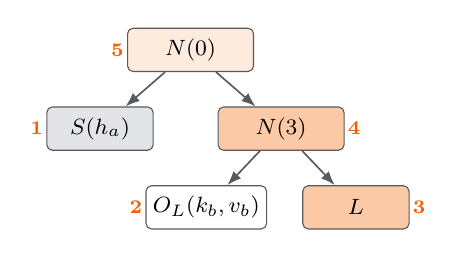
\begin{tikzpicture}[x=1cm,y=1cm]
  \node[jn, fill=recomp, label={[ord]left:5}] (n) at (0,0) {$N(0)$};
  \node[lf, fill=preserved, label={[ord]left:1}] (na) at (-1.15,-1.0) {$S(h_a)$};
  \node[jn, fill=fresh, label={[ord]right:4}] (nj) at (1.15,-1.0) {$N(3)$};
  \node[lf, fill=opened, label={[ord]left:2}] (nb) at (0.2,-2.0) {$O_L(k_b,v_b)$};
  \node[lf, fill=fresh, label={[ord]right:3}] (nc) at (2.1,-2.0) {$L$};
  \draw[arr] (n) -- (na);
  \draw[arr] (n) -- (nj);
  \draw[arr] (nj) -- (nb);
  \draw[arr] (nj) -- (nc);
\end{tikzpicture}\\[1mm]
\scriptsize
\swatch{preserved} opaque\quad \swatch{opened} opened\quad \swatch{fresh} new\quad \swatch{recomp} re-hashed\\[1mm]
{\footnotesize (a)}
\end{minipage}\hfill
\begin{minipage}[b]{0.5\textwidth}\centering
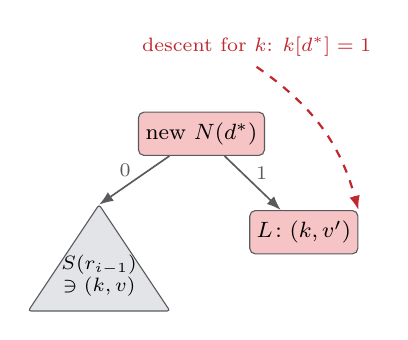
\begin{tikzpicture}[x=1cm,y=1cm]
  \node[jn, fill=attack] (n) at (0,0) {new $N(d^*)$};
  \filldraw[fill=preserved, draw=lineGrey, rounded corners=1pt] (-1.3,-0.9) coordinate (apex) -- (-2.2,-2.25) -- (-0.4,-2.25) -- cycle;
  \node[font=\scriptsize, align=center] at (-1.3,-1.8) {$S(r_{i-1})$\\$\ni (k,v)$};
  \node[lf, fill=attack] (l) at (1.3,-1.25) {$L\colon (k,v')$};
  \draw[arr] (n) -- node[bitlbl, above left] {0} (apex);
  \draw[arr] (n) -- node[bitlbl, above right] {1} (l);
  \draw[-{Latex[length=1.8mm]}, attackline, thick, dashed] (0.7,0.85) node[above, font=\scriptsize] {descent for $k$: $k[d^*]=1$} to[bend left=20] (l.north east);
\end{tikzpicture}\\[1mm]
{\footnotesize (b)}
\end{minipage}
\Description{Left: transcript tree with root N(0) over the opaque subtree S(h_a) and the new junction N(3); N(3) is over the opened leaf O_L(k_b, v_b) and the new leaf L. Post-order numbers 1 to 5 label S, O_L, L, N(3), N(0). Right: a new junction at depth d* with the whole pre-state tree as an opaque subtree on its 0-side and a new leaf (k, v') on its 1-side; the descent for k, which has bit 1 at depth d*, leads to the new leaf.}
\caption{(a) Transcript for the insertion of Fig.~\ref{fig:insert}; numbers give the post-order. (b) A transcript that passes all digest checks under a junction hash that commits to the depth only (Remark~\ref{rem:placement}). It is rejected by confinement and edge coherence.}
\label{fig:batch}
\end{figure}

\begin{table}[t]
\centering
\caption{Verification of the transcript in Fig.~\ref{fig:batch}a.}\label{tab:trace}
\footnotesize
\setlength{\tabcolsep}{4pt}
\begin{tabular}{@{}lllll@{}}
\toprule
& Opcode & Pre-state digest & Post-state digest & Advice \\
\midrule
1 & $S(h_a)$ & $h_a$ & $h_a$ & $\bot$ \\
2 & $O_L(k_b,v_b)$ & $h_b$ & $h_b$ & $(\kappa, k_b)$ \\
3 & $L$ & $\varnothing$ & $h_c$ & $(\kappa, k_c)$ \\
4 & $N(3)$ & $h_b$ & $h_N = \NodeHash(3,\bits{110},h_b,h_c)$ & $(3,\bits{110})$ \\
5 & $N(0)$ & $\NodeHash(0,\varepsilon,h_a,h_b) = r_{i-1}$ & $\NodeHash(0,\varepsilon,h_a,h_N) = r_i$ & $(0,\varepsilon)$ \\
\bottomrule
\end{tabular}
\end{table}

\begin{remark}[Placement]\label{rem:placement}
Preserving the hashes of the pre-state does not preserve the dictionary. Suppose the junction hash committed to the depth only and the verifier checked only the digest algebra. Let $(k,v)$ be recorded under $r_{i-1}$ and pick $d^*$ with $k[d^*] = 1$. The stream $[S(r_{i-1}), L, N(d^*)]$ with batch $\{(k,v')\}$, $v' \neq v$, passes all digest checks: the pre-state side passes $r_{i-1}$ through, and the post-state side hangs the whole pre-state tree on the $0$-side of a new junction (Fig.~\ref{fig:batch}b). The descent for $k$ under $r_i$ takes the $1$-side, so $(k,v')$ has an inclusion certificate against $r_i$ and $(k,v)$ has none. The verifier above rejects the stream: confinement requires the preserved child of the new junction to be opened, and edge coherence then requires its region to extend $p \cat \bits{0}$, which is impossible because that region is a prefix of $k$ and $k[d^*] = 1$.
\end{remark}

\begin{definition}[Certified history]\label{def:history}
A \emph{certified history} is a sequence $(B_1,\pi_1,r_1),\ldots,(B_n,\pi_n,r_n)$ with $r_0 = \varnothing$ such that the verifier accepts $(\pi_i, r_{i-1}, r_i, B_i)$ for every $i$. With $M_0 = \emptyset$ and $M_i = M_{i-1} \uplus B_i$, the history is \emph{append-only consistent} if every disjoint union is defined and $r_i = \dig(\Tree(M_i))$ for all $i$.
\end{definition}

\begin{theorem}[History soundness]\label{thm:history}
Every certified history is append-only consistent.
\end{theorem}
\begin{proof}[outline]
By induction on rounds it suffices to show: if $T$ is a valid tree with $\dig(T) = r_{i-1}$ and the verifier accepts $(\pi, r_{i-1}, r_i, B)$, then there is a valid $T'$ with $\dig(T') = r_i$ and $\map(T') = \map(T) \uplus B$; Proposition~\ref{prop:unique} then gives $T' = \Tree(M_i)$. The argument has three steps~\cite{fullversion}. (1)~An accepted stream is the post-order serialization of a unique proof term, on which the three checks become a local predicate. (2)~Removing the $L$ leaves and collapsing new junctions turns the term into an opening tree that evaluates to $r_{i-1}$, so Lemma~\ref{lem:match} places every $S$, $O$, and $O_L$ in $T$. (3)~Grafting the matched subtrees of $T$ into the term yields $T'$ with $\dig(T') = r_i$. Every edge of $T'$ is either an edge of $T$ or has an advised child that passed the coherence check; confinement excludes an opaque subtree under a new junction. Thus $T'$ is valid, its leaf keys are distinct by Lemma~\ref{lem:shape}(i), the keys of $B$ are fresh, and $\map(T') = \map(T) \uplus B$.\qed
\end{proof}

\begin{theorem}[Completeness]\label{thm:complete}
For a valid $T$ and a batch $B$ of distinct keys absent from $\map(T)$, a transcript that the verifier accepts for $(\dig(T), \dig(\Tree(\map(T) \uplus B)), B)$ is computable in time linear in its length after sorting $B$.
\end{theorem}

\begin{corollary}\label{cor:history}
In a certified history: inclusion certificates for $(k,v)$ against $r_i$ and for $(k,v')$ against $r_j$ imply $v = v'$; once a certificate for $k$ with terminal key $k$ verifies against $r_i$, no certificate for $k$ with another terminal key verifies against any $r_j$, $j \ge i$; and an inclusion certificate for $(k,v)$ against $r_i$ implies $(k,v) \in B_1 \uplus \cdots \uplus B_i$.
\end{corollary}

% =====================================================================
\section{Implementation}\label{sec:impl}
% =====================================================================

The data structure scaling experiments with respective proof verifiers are available as human-readability optimized Python code\cite{ndsmtexp}, and the production aggregator is implemented in Rust with a disk-backed RSMT~\cite{rugregator} . At $10^6$ leaves, the transcript and batch take about 320 bytes per insertion, so with the plain transcript the Consensus Layer receives data in proportion to the transaction rate, eventually becoming the scaling bottleneck. A custom AIR on Plonky3 Zero Knowledge framework~\cite{plonky3,rsmtair} proves the verifier of Sect.~\ref{sec:batch} with the batch as witness data and $(r_{i-1}, r_i)$ as public input. With Poseidon2 as the tree hash, one consumer CPU proves more than $10^4$ insertions per second per shard; a proof of about 1.8\,MB verifies in under 50\,ms independent of the batch size. This the first practical use of Zero Knowledge (as a computational integrity tool), in a high-performance transaction system, known to the authors. Horizontal scalability is achieved by sharding. A key prefix selects the shard, and a shard can be further split on-the-fly without rehashing because each child root is an existing subtree. The extended version of the paper describes the AIR, the sharding scheme, and the recursive STARK over all rounds~\cite{fullversion} to achieve a compact cryptographic  proof of history correctness of the Unicity Infrastructure.

% =====================================================================
\section{Related Work}\label{sec:related}
% =====================================================================

Certificate Transparency~\cite{rfc6962} and tamper-evident history trees~\cite{crosby2009} provide consistency proofs between successive heads of a chronological Merkle log. A log has no key-determined positions, so a second entry for the same key is not excluded by the proof. In a keyed dictionary a double-spend is a key collision, which the consistency proof excludes. Authenticated dictionaries with accountability were studied by Buldas, Laud, and Lipmaa~\cite{buldas2000}; CONIKS~\cite{melara2015} uses prefix trees for key directories, and Reyzin et al.~\cite{reyzin2017} give authenticated dynamic dictionaries for cryptocurrencies. Append-only authenticated dictionaries by Tomescu et al.~\cite{tomescu2019} use bilinear accumulators and require a trusted setup. Sparse Merkle trees with efficient (non-)membership proofs are studied in~\cite{dahlberg2016smt}. Our tree is a hash-only Patricia trie whose junction hash commits to the region, which keeps certificates at the depth-only size and makes placement locally checkable in the consistency proof.

Zerocash~\cite{zerocash} and its descendants maintain a nullifier set, and each spender proves knowledge of an unspent note in zero knowledge. Validity rollups such as Polygon zkEVM~\cite{polygonzkevm} prove the execution of all transactions of a block. Both put execution or user secrets into the proved statement. Our consistency proof covers only the dictionary update, and its size depends on the batch and logarithmically on the tree. A single-assignment register per key is a sticky bit, a universal primitive for consensus objects~\cite{plotkin1989}; any state machine with provable transitions can be advanced with a uniqueness guarantee by keying registers with (object, sequence number).

% =====================================================================
\section{Conclusion}\label{sec:conclusion}
% =====================================================================

The online part of a trustless peer-to-peer token system reduces to an add-only dictionary of consumed states. The region-committing RSMT implements it with certificates of near-optimal size that serve both inclusion and non-inclusion. A non-inclusion certificate is a consistency proof for one insertion, and batch transcripts are sound once placement is checked locally at every created edge. In both cases the security of the whole certified history reduces to collision resistance of the hash function. A machine-checked formalization of the proofs is future work.

\begin{credits}
\subsubsection{\discintname}
% TODO: Springer requires a disclosure of interests statement.
\end{credits}

\bibliographystyle{splncs04}
\bibliography{references}

\end{document}
